\section{Compression Related Tasks}


\subsection{Text Compression as Translation}


{For the NLP tasks of text compression and text simplification, an expedient way to make progress towards a working system has been to adapt existing methods from other NLP tasks.  In the case of text compression, the noisy channel model has been a promising method used by several different researchers because of it's suitability to tasks which require a conversion from one string to another \citep{knight2000statistics,galley2007lexicalized}. In this sub-section we will discuss the theoretical underpinnings of a Noisy Channel model as proposed by \citet{knight2000statistics} and then shift our attention to some improvements by \citet{galley2007lexicalized} which builds off of Knight and Marcau's system by adding variable levels of lexical and phrase based information. This sub-section is intended to give the reader a close look at some data driven approaches to text compression which operate only on the sentence. From this starting point we can later explore how the noisy channel model relates to some text simplification systems, and how it diverges from discourse based systems in both compression and simplification.}

{\citet{knight2000statistics} were some of the first researchers to propose the noisy channel model as a solution to the compression problem.  In their paper they provide a thorough and illustrative description of how the noisy channel works in general, which serves as the conceptual grounding for their system, as well as the system by \citet{galley2007lexicalized}.  In the paper, the authors assume that a short string (the ideal compression) is transmitted over a channel and at the other end a long string (the un-compressed message) is received.  Because the channel for transmitting the message is noisy, the original short message is corrupted and ends up being transformed into the long message which can be observed. The goal is to reason backwards from the observed string as to what is the most likely short string which created it (see figure \ref{fig:channel}).  In other words if $ c $ is a compression in the set of all grammatical compressions $C$, and $ f $ is the full text observed, then one is trying to find $ \hat{c} = argmax_{c\in C} \{ p(c|f)\} $.  This equation can be further broken down into a \textbf{translation model} and a \textbf{language model} as in the case of\citet{knight2000statistics}, or in the case of \citet{galley2007lexicalized} the two models are collapsed into one single translation model for purposes of easier computation within their framework.}

\begin{figure}[H]
\centering
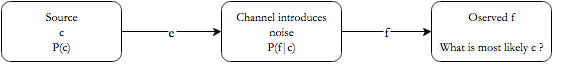
\includegraphics[width=0.8\textwidth]{noisyCh.png}
\caption{The noisy channel pipeline.}
\label{fig:channel}
\end{figure}


{In any implementation of the noisy channel model, the translation model is the key to describing the probability that one string is transformed into another across the channel.  In a classic example of the noisy channel model for machine translation, obtaining these probabilities is a well established task of collecting counts of aligned words in order to predict the probability of a translation.  However, because word deletion can be difficult to accurately model in  translation, this approach was deemed inadequate to represent sentence compression.  In order to solve this problem, \citet{knight2000statistics} instead use a syntax based approach which models a translation between sub-trees described by a \textbf{Synchronous Context Free Grammar} (SCFG).  SCFGs can be defined as context free grammars whose productions have two right hand side rules, one representing the source constituents, and the other representing the target constituents, which in the case of text compression will be some sub sequence of the source side \citep{galley2007lexicalized}. The following is an example of a deletion rule in a SCFG for removing a prepositional phrase:}

\begin{figure}[H]
\centering
VP $ \rightarrow  \langle$ VBD PP PP, VBD PP $\rangle$
\caption{An example rule from an SCFG}
\label{fig:scfg}
\end{figure}

{In order to train a SCFG language model, parallel sentences must be obtained from a corpus in order to observe where deletions happen and  obtain counts of them to estimate their likelihood.  Both papers used the Ziff-Davis corpus which is a collection of technical documents paired with abstracts. \citet{knight2000statistics} only use a small fraction of the corpus ($1.75 \%$ of abstract sentences), because they follow the strict definition of compression as a series of word deletions, and this means they can only include sentence pairs where the compressed sentence is an exact subset of words from the source sentence.  Furthermore, of the small fraction of the corpus being used, they can only train rules for the grammar when there is a clear alignment between sub-trees in the source and compression sentences.  This leaves them with a rather small set of data to train their system on.  \citet{galley2007lexicalized} decide to loosen their criteria of sentence compression and allow for a limited number of word substitutions edits in addition to word deletions.  This provided a much larger set of training data (up to $25 \%$ of summary sentences when allowing 6 substitutions per sentence).   It's interesting to note that if even more edit rules were allowed in training the system, such as insertion, or re-ordering, the resulting SCFG rules would be moving away from a model of pure compression towards something more like text simplification.  This shows that sentence compression could be thought of as a special case of simplification.}


{By using SCFGs, the papers make some implicit assumptions about what kind of information will play a role in deleting words from a source sentence.  For instance, the focus on deletion of constituents rather than words makes the system blind to any lexical information which may bias towards retaining or deleting a constituent from a sentence. To improve upon this \citet{galley2007lexicalized} decided to expand the annotation in their SCFGs by tagging the lexical head and POS of a syntatic category.  By adding lexical head information the system can more accurately predict for instance, that some PP's are compliments of a verb (and likely to be preserved) while other PP's are adjuncts and better candidates for deletion (see figure \ref{fig:tree}).}

\begin{figure}[H]
\centering
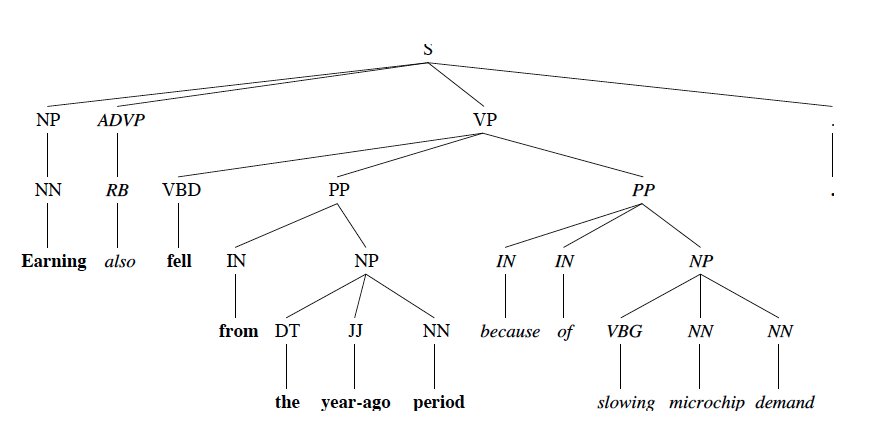
\includegraphics[width=0.7\textwidth]{tree1.png}
\caption{a penn treebank example of PP compliment and PP adjunct.}
\label{fig:tree}
\end{figure}

{The authors are also interested in using embedding depth to predict the importance of a constituent.  In order to model this, they add annotation to label the parents of constituents to varying depth, for example an NP beneath a PP, VP, and S parent node would be labeled NP\^{}PP\^{}VP\^{}S with an embedding depth of 3.  They assume that constituents embedded deep within a PP, for example, would be good candidates for removal based on their position and depth in the sentence.  This idea of phrase embedding depth also plays an important role in the next system being discussed, although used in a slightly different manner.  While these extra features were found to improve the  accuracy of the \citet{galley2007lexicalized} model above \citet{knight2000statistics}, it is important to mention that both systems are only compressing individual sentences, and base their deletion decision almost exclusively on syntactic information. As one can imagine, there are many situations where text compression may benefit from more information than just parse trees. Concepts like word frequency scores, lexical relations, and sentence "centers" may all contribute to a more nuanced and cohesive compression that what has been presently discussed.  These concepts and more will be explored in the next sub-section, which will cover a discourse driven approach to text compression.}




\subsection{Text compression With Discourse Constraints}
  

{The conceptual framework for the compression system used by \citet{Clarke:2010:DCD:1950488.1950493} diverges significantly from the noisy channel systems in the previous sub-section.  the authors re-imagines the task as an optimization problem:  Given a string of text, retain the words which maximize a scoring function.  The scoring function is bound by a series of competing constraints, including rules about enforcing grammaticality, keeping text to a certain length, and retaining informative words based on sentence and discourse level information \citep{Clarke:2010:DCD:1950488.1950493}.  In order to solve for the optimal score, the scoring function and constraints are represented as linear inequalities and are evaluated by \textbf{Integer Linear Programming} (ILP).  ILP can be thought of as a type of general problem solver tool which efficiently searches for an optimal integer solution to linear functions.  This approach frees up the system to perform more flexible compression than was possible in the noisy channel approach. This allows for more variable compression rates, compressions of text of arbitrary length (rather than just sentences), and the ability to model any important information for compression, such as discourse information, as a constraint to the scoring function.} 

{The first part of the scoring function is a significance score aimed to boost the value of topic related words (assumed to be nouns and verbs).  The significance score attempts to get the gist of how important a word is the context of the document, and the sentence.  The first part of the significance equation is something similar to  \textbf{tf} $ \bullet $ \textbf{idf}, and compares the word's document frequency to it's frequency in a training corpus of similar documents and determines it's relative importance.  The second part of the equation gives more importance to words based on the depth of \textbf{embedding} of the clause they are found in.  The intuition from the authors is that a content word in a deeply embedded clause carries more semantic content, and thus should have higher chances of retention.  This representation of an embedding score is quite different from the example by \citet{galley2007lexicalized} who measured constituent depth rather than clause depth. But it shows that in both cases, looking at where a word lies in the 'vertical' space of a parse can be helpful to determine it's importance to the final compression.}

{Next, the backbone of the scoring function is a language model of candidate compressions which operates in tandem with a set of constraints.  The language model calculates a score for all  candidate compressions, while the constraints dictate which compressions are vailid, and penalize/reward certain compressions based on syntax and discourse content \citep{Clarke:2010:DCD:1950488.1950493}. The first set of constraints on the language model are to ensure that any candidate compression is a well formed in the most basic technical sense, meaning that the sentence has a start and end point, and than only one word occupies each position in the sentence.  The next set of constraints are sentence level syntactic constraints developed by the authors in a previous paper \citep{Clarke:2008:GIS:1622655.1622667}.  These constraints are hand coded rules intended to preserve the meaning and structure of the original sentence as much as possible.  The rules in general describe situations where if a certain element is included (negations, adjectives, adverbs, determiners, prepositions) than the head of that element must also be included so it's not left floating in a sentence without context. As an example, if an argument is present in the compression, than the verb to which that argument belongs must also be included.  This bottom up approach to retaining constituents contrasts with the previous papers which had a top down deletion rule as illustrated by figures (\ref{fig:tree}) (\ref{fig:scfg}). The choice to use hand coded syntax rules rather than a data driven approach means the system may miss some useful syntax rules derived from the data, but is more insulated from "noisy" rules which are observed very infrequently.}

{The third set of constraints are related to discourse information and are used to prioritize retention of words which support coherence within the document.  Coherence is an important concept in discourse which relates to the overall intelligibility of the message in a text.  Because global coherence is quite difficult to model automatically (attempts have been made using Rhetorical Structure Theory ***CITE), the authors instead use two complimentary theories of discourse which attempt to model local cohesion as a proxy for global coherence.  The first theory is \textbf{lexical chains}, which can be thought of as groups of semantically related words from the document which represent lexical cohesion (Morris and Hirst 1991).  Main topics for the paper are identified as long lexical chains with strong semantic relation among them (see figure \ref{fig:centering}).  The next discourse theory used is \textbf{centering theory}.  This theory operates on the idea that within a sentence, there exists an entity which is more salient than the others and considered the focus of the sentence. The center is identified according to it's grammatical function, and it's relation to entities in the preceding and following sentences (see figure \ref{fig:centering}). In using these discourse constraints to retain words which show high cohesion, the system in effect also gains a secondary grammar check which strongly rewards retention of the subject and objects in a sentence.}


\begin{figure}[H]
\centering
\begin{scriptsize}
Bad weather dashed hopes of attempts to halt the $flow_{1}$ during what was seen as a lull in the \textbf{lava's} momentum. Experts say that even if the eruption stopped $today_{2}$ , the pressure of \textbf{lava} piled up behind for six $miles_{3}$ would bring \textbf{debris} cascading down on the town anyway. Some estimate the volcano is pouring out one million tons of \textbf{debris} a $day_{2}$ , at a $rate_{1}$ of 15 $ft_{3}$ per $second_{2}$ , from a fissure that opened in mid-December.
The Italian Army $yesterday_{2}$ detonated 400lb of dynamite 3,500 feet up Mount Etna’s slopes.
\end{scriptsize}

\caption{lexical chains are listed in italics with sub-script and centers are written in bold}
\label{fig:centering}
\end{figure}

{The use of discourse information in many NLP tasks at present still faces a challenge of reliably and accurately identifying the elements relevant to discourse.  This paper provides a good example of applying discourse information in a manageable scale, such as searching for local cohesion, rather than attempting to define the global discourse structure of the whole document.  The system is also designed in such a way that training data comes from a single corpus, rather than needing aligned pairs of source and compression sentences.  This design is much more insulated against issues of sparse data as seen in the previous examples from \citet{galley2007lexicalized} and \citet{knight2000statistics}.  This is an important consideration for any compression or simplification system, considering that quality results may be more limited by available data rather than any flaw in the design of the model itself.}


\subsection{Simplification with Discourse Constraints}



{Moving now from text compression to text simplification, the first example being presented is from the a paper by \citet{Siddharthan2006}.  The system described in this paper is designed to reduce the syntactic complexity of a document while also trying to retain text cohesion.  The author motivates the use of discourse level information for the task by pointing out several problems which can arise from compression or simplification without discourse information.  The first concern is that a loss of cohesion could make the text more difficult to comprehend, which in effect, is the opposite of what simplification systems aim to achieve. A system blind to discourse information also runs the risk of changing the intended meaning.  This concern is echoed in the previous system which also tries to achieve better coherence in the compression by use of lexical chains and centering theory.}

{The scope of simplification as presented in this paper is to divide long sentences into smaller sentences, and then to resolve issues of cohesion through sentence reordering and addressing pronominal links. The architecture of the system is divided into 3 steps:  \textbf{analysis, transformation,} and \textbf{regeneration} (see figure \ref{fig:architecure} for an illustration of the architecture).  In the analysis stage, markup is performed on the text for sentences boundaries, POS tags, noun chunks, pronoun resolution, and boundaries and attachment for clauses/phrases.  This step is pre-processing so that the transformation stage can apply rules for breaking up a sentence into sub-sentences.  Each time a sentence is split, it's sent to the regeneration stage to address issues of conjunctive cohesion such as sentence order, referring expressions, and adding cue words.  The transformation stage is repeated recursively, meaning that each sub-sentences is placed back on the stack of sentences to split until no further splitting rules apply.  All minimally reduced sentences are passed one final time to a different part of the regeneration stage, at which point anaphoric cohesion is resolved.}

\begin{figure}[H]
\centering
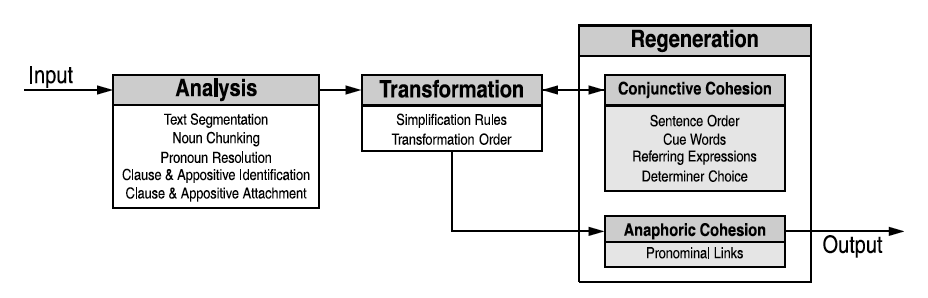
\includegraphics[width=0.7\textwidth]{arch.png}
\caption{the architecture of the Siddharthan system.}
\label{fig:architecure}
\end{figure}


{The rules for how sentences are split in the transformation phase are hand written and are similar to a Context Free Grammar.  However this rule set differs from the SCFG seen in \citet{knight2000statistics} because it doesn't require the synchronous aspect with two parallel right hand side rules. To illustrate, the rule displayed in figure \ref{fig:simprule} shows a sentence comprised of parts $V W X Y Z$ where $W$ is a noun phrase and $Y$ is a relative clause attached to the noun in $W$.  The rules states that the sentence can be split into sub sentences $(i)$ and $(ii)$, and are linked by the relation $RELPR$.  Each time a sentence is split, the resulting form is a triplet $(a, R, b)$ which shows one reduced sentence $a$ as a nucleus connected to the other reduced sentence $b$ by relation $R$.  The creation of the rule set with relations and the use of nucleus/satellite terminology is based on  \textbf{Rhetorical Structure Theory} (RST), which is a comprehensive discourse theory used to describe how sentences relate to one another across a document \citep{•}.  Because parsing a text for it's RST structure as a pre-processing step is too noisy and un-reliable to use directly, here the author chooses a more tractable task of matching phrases in a sentence to a set hand picked rhetorical relation rules relevant just to sentence splitting.}

\begin{figure}[H]
\centering

$ \langle s \rangle V W^n_{NP} [_{RC} RELPR^{\#n}Y]Z. \langle s \rangle \rightarrow \begin{aligned} (i) \langle s \rangle V W X Z.  \langle /s \rangle \\ (ii)  \langle s \rangle W Y. \langle /s \rangle \end{aligned}  $

\caption{a simplification rule for the system by Siddharthan.}
\label{fig:simprule}
\end{figure}


{Once sentences have been split by a rule in the transformation stage, they must be properly ordered to maintain coherence.  For the sake of simplicity, re-ordering occurs locally each time a sentence is split, rather than globally for all sub sentences at once.  At each re-ordering stage, the triplet $(a, R, b)$ is provided, along with an inherited set of hard and soft constraints $ C $ introduced from any prior transformations. If the relation between the sentences adds any new constraints on re-ordering, those constraints are also added to $C$.  While the list of constraints is too long to describe here in full detail, an example of a re-ordering based on a centering theory constraint is provided in figure \ref{fig:cent-theory}). The example shows a preference for version b which has a cohesive "retaining" transition from sentence 1 to 2, rather than a "shift" transition as shown in b (see \citet{grosz1995centering} for more on centering theory transitions).}


\begin{figure}[H]
\centering
\begin{footnotesize}

a.  They will remain on a lower priority list that includes 17 other countries.

b. (1) They will remain on a lower-priority list.  (2) This list includes 17 other countries.

b' (1) A lower-priority list includes 17 other countries.  (2) They will remain on this list.

\end{footnotesize}
\caption{an exmaple of re-ordering based on centering theory.}
\label{fig:cent-theory}
\end{figure}

{As one may notice from the architecture and constraints described above, the system by \citet{Siddharthan2006} is entirely rule based and does not require any training data.  This skirts the issue of error due to insufficient data by basing rules on established principles of discourse and syntactic theory.  As a draw back, it makes the expansion or editing of the system much more brittle and labor intensive.  For the limited scope of simplifying text by splitting up sentences this may be sufficient, but if other elements such as semantic simplification were to be added, one would imagine that a data driven element such as seen in the translation based systems would be helpful.  Another drawback to this system is that it only performs simplification on a sentence by sentence basis.  While it does consider maximizing coherence in doing so, it might be advantageous to be able to perform sentences reordering and pronoun reference resolution in a larger context to further improve readability and cohesion.} 


\subsection{Simplification as Translation}

{The final example of a system for text simplification will bring the focus back to use of translation as a framework.  The paper from   \citet{coster-kauchak:2011:T2TW-2011} proposes a phrase based translation system for text simplification which has been trained on a parallel corpus of standard English and simple English Wikipedia articles.  The use of Wikipedia articles for training the system provided a data set of 137k aligned sentences \citep{coster-kauchak:2011:T2TW-2011}, which is orders of magnitude larger than the sentence pairs from the Ziff Davis corpus used by \citet{knight2000statistics} and \citet{galley2007lexicalized}.  This large amount of data is promising because it offers a much more robust statistical model of translations than what was seen in the compression examples.}

{In order to generate the corpus of aligned normal and simple sentences several steps were taken to extract suitable pairs.  First normal and simple wiki articles were matched based on exact title.  From there, paragraphs were aligned based on TF-IDF cosine similarity above a certain threshold.  Sentences from the aligned paragraphs were then sorted into groups depending on whether they had a one to one alignment,  one to two alignment, or were inserted/deleted.  Sentences which had positive alignments were then compared again on TF-IDF cosine similarity and only those which were over a threshold were kept as alignments\citep{coster-kauchak:2011:T2TW-2011} .}  

{From these aligned sentence pairs, the  phrase based machine translation system (PBMT) is then ready for training.  One can think of a PBMT as an extension of the noisy channel model with a langauge and translation model, but rather than the translation model being based on individual words or SCFG rules, it uses phrases to capture interactions which occur within a sequence of words.  The formula for the model can be written as:
\[\hat{c} = p(c|f) = \prod^m_{i=1} p(\bar{c_i}|\bar{f_i})\]
With $c$ representing the compression sentence, and $f$ representing the full sentence and $c_i , f_i$ being phrases consisting of 1 or more contiguous words. The convenience of using phrases for the task of simplification is that a transformation from one small sequences of words to another can automatically capture several types of simplification operation such as rewording, reordering, and insertion. However, most PBMT systems out of the box cannot easily model the deletion operation because it may complicate the decoding process.  Therefore The authors decided to modify the Moses system by \citet{koehn2007moses} to allow for phrases from the simple sentences to be empty, and added the probabilistic phrasal deletion rule $p(NULL|\bar{n_i})$ which would represent this deletion.}  

{Another interesting improvement added during the testing stage of the system was to use an oracle which searches a beam of the 1000 best simplifications output and select the one which scores highest by a ranking metric such as BLEU \citep{{papineni2002bleu}.  This is a exciting suggestion which could not only improve this specific task, but could also possibly be ported to compression systems mentioned earlier. Finally, it should also be pointed out a few drawbacks noticed in the design of this system. To start, aside from the special case of deletion, all the other edit operations are collapsed into the single task of translation.  This makes it difficult if not impossible to individually parameterize what types of edits should be preferred or discouraged.. In addition, the lack of information beyond the sentence level means that entities which are re-named or deleted in one sentences could appear in the next with no clear mention of what was originally being referred to. }






 recgonize the need for several edit operations in order to 
